\chapter{Projektstruktur und -organisation}
\label{sec:orga}
\marginpar{Benjamin}

In der ersten Woche der Projektgruppe wurde eine Seminarphase durchgeführt in
der die theoretischen Grundlagen des Themas sowie Grundlagen des
Projektmanagements und der Softwareentwicklung erarbeitet. Im Anschluss wurde in
der Projektgruppenordnung festgehalten, wie die Projektgruppe weiter verlaufen
wird. In der Seminarphase stellten sich folgende Tools als besonders geeignet
heraus um den weiteren Ablauf der Projektgruppe zu organisieren:

\begin{itemize}
    \item Scrum als Vorgehensmodell für die Projektgruppe.
    \item Redmine als Ticketsystem zur Verwaltung der Aufgaben und deren
      Verteilung, sowie als Wiki zum festhalten von Protokollen und
      organisatorischen Informationen.
    \item git für die Versionierung und Verwaltung des Quellcodes.
\end{itemize}

\section{Projektmanagement}
\label{sec:orga:projekt}
\marginpar{Benjamin}

Im Projektmanagement kommt es vor allen Dingen darauf an, dass klare
Aufgabendefinitionen und das setzen eindeutige Start- und Endtermine ist
unerlässlich. Die Ziele der Projektgruppe stehen im Vordergrund und müssen klar
strukturiert und verständlich heruntergebrochen werden, sodass ein
funktionierendes Miteinander gewährleistet ist. Um das Projektgruppe-Ziel zu
erreichen müssen Bestimmungsgrößen Ziel, Zeit und Ressourcen entsprechend
heruntergebrochen werden, um sie so auf die Teilnehmen zu verteilt.
Standardvorgehensmodelle bieten einen gewissen Aufbau mit dem sich die
Projektgruppe gezielt organisieren kann. Die Projektgruppe identifizierte jedoch
auch gewisser Kernelemente die auch über das Vorgehensmodell hinaus Geltung
finden.  Diese Elemente sind:

\begin{itemize}
  \item Verwaltung und Identifizierung der Arbeitsschritte
  \item Gezieletes Aufteilen in klare verständliche Arbeitspakete.
  \item Effiziente Arbeits- und Arbeitslastenverteilung,
  \item Rege Kommunikation,
  \item Transparenz - Offenes Kommunizieren der Fähigkeiten und des Fortschritts
  \item Fortlaufende Dokumentation
\end{itemize}

\subsection{Rollen der Projektteilnehmer}
\label{sec:orga:projekt:rollen}
\marginpar{Benjamin}

In der Projektgruppenordnung wurden vier spezielle Rollen festgeschrieben und mit jeweils einer Person besetzt. Dabei handelt es sich um den

\begin{description}
\item[Projektleiter,] der die Verantwortung für das Projekt übernimmt und die
Arbeitsfortschritte überwacht. Er leitet jede Sitzung der Projektgruppe und
achtet auf die Einhaltung der Tagesordnung, der Projektleiter übernimmt außerdem
die Aufgaben eines ScrumMasters, der die wöchentlichen Fortschrittsberichte
koordiniert. Bei Abstimmungen mit Stimmengleichheit entscheidet der
Projektleiter.

\item[Protokollant] führt über jede Sitzung ein Protokoll. Dieses wird im
Redmine-Wiki hinterlegt und enthält die Namen der Anwesenden, die
Tagesordnungspunkte, Informationen zu eventuell abgehaltenen Abstimmungen und
sonstige abgegebene Erklärungen.

\item[Teamleiter] erstellt und weist Tickets im Redmine zu. Darüber hinaus
kümmert er sich um die Administration des Redmine-Systems.

\item[Berichtmanager] sorgt für die Einhaltung von Deadlines, die den Bericht
betreffen, erstellt Vorlagen und sichert die Qualität des Berichts durch
Einhaltung von formalen und inhaltlichen Kriterien.
\end{description}

\subsection{Scrum}
\label{sec:orga:projekt:scrum}
\marginpar{Benjamin}

Das Projektmanagement für die Projektgruppe lehnt sich an das Scrum-Framework
an. Scrum ist ein agiles Vorgehensmodell zur Softwareentwicklung, in dem der
Zeitraum in Sprints aufgeteilt werden. Diese Sprints sind maximal einen Monat
lang und sorgen für eine inkrementelle Erweiterung des Projekts.

\begin{itemize}
\item Transparenz: Der Projektfortschritt wird in \textit{daily scrums} jeden
  Tag für jedes Teammitglied sichtbar festgehalten.
\item Überprüfung: Durch die Sprints wird in regelmäßigen Abständen ein Ergebnis
  erzielt und am Ende eines Sprints kann dieser von den Teammitgliedern bewertet
  werden.
\item Anpassung: Die Planung wird kontinuierlich erweitert und verbessert.
\end{itemize}

In der Projektgruppe wird der Projektfortschritt wöchentlich besprochen, der
Projektleiter organisiert dies. Wir haben desweiteren die zwei Semester der
Projektgruppe in insgesamt 5 Sprints aufgeteilt. Die jeweils $5-7$ Wochen lang
sind.

\begin{figure}[htb]
\begin{center}
\begin{ganttchart}{1}{12}
\gantttitle{2014}{9}
\gantttitle{2015}{3} \\
\gantttitlelist{4,...,12,1,2,3}{1} \\
\ganttbar{Sprint 1}{1}{2} \\
\ganttbar{Sprint 2}{3}{4} \\
\ganttbar{Sprint 3}{7}{8} \\
\ganttbar{Sprint 4}{9}{10} \\
\ganttbar{Sprint 5}{11}{12}
\ganttlink{elem0}{elem1}
\ganttlink{elem1}{elem2}
\ganttlink{elem2}{elem3}
\ganttlink{elem3}{elem4}
\end{ganttchart}
\end{center}
\caption{Übersicht Sprintplanung}
\label{fig:sprintplanung}
\end{figure}

\begin{description}
  \item[1. Sprint] (6 Wochen) dient der Aneignung der Theoretischen Teile, des
    Herausarbeitens der Programmstruktur und welche Algorithmen eingesetzt
    werden sollen sowie der Implementierung eines einfachen Prototypen aus dem
    unser Readmapper dann weiterentwickelt werden kann.
  \item[2. Sprint] (7 Wochen) zur Implementierung des Readmappers und zur
    Erstellung des Zwischenberichts. Auf diesen Sprint folgt mit der
    vorlesungsfreien Zeit eine längere Pause.
  \item[3. Sprint] (6 Wochen) hier sollen Benchmarks ausgeführt werden, das
    Finden neuer Varianten implementiert sowie eine grafische Oberfläche für
    unser Programm entworfen werden.
  \item[4. Sprint] (5 Wochen) ist gedacht für weitergehende Experimente und den
    Beginn der Auswertung.
  \item[5. Sprint] (5 Wochen) finale Auswertung und Erstellung des Endberichts.
\end{description}

\subsection{Redmine}
\label{sec:orga:projekt:redmine}
\marginpar{Benjamin}

Zur Organisation wurde die Redmine-Installation des ITMC benutzt. Die
wesentlichen genutzten Funktionen dieses Systems sind das Wiki, in dem die
laufenden Dokumentation der Projektgruppe festgehalten wird. Dies Umfasst die
wöchentlichen Protokolle, die Projektgruppenordnung und Informationen zur
verwendeten Literatur. Im Ticketsystem wird dokumentiert, welche Aufgaben von
wem wann bearbeitet werden sollten. Dazu kann auch eine Kalenderansicht
aufgerufen werden in der die Tickets zeitlich dargestellt werden. Des weiteren
bietet Redmine ein Webinterface zur Ansicht der Änderungen in einem Veknüpften
git-Repository. Tickets und Änderungen im git können sich gegenseitig
referenzieren. Das Redmine-System wird vom Teamleiter gepflegt, insbesondere
sorgt er für eine regelmäßige Aktualisierung der Tickets.

\section{Versionsverwaltung mit git}
\label{sec:orga:vers}
\label{sec:orga:vers:git}
\marginpar{Kada}

Git ist ein Versionierungstool zur Codeverwaltung.

Git wurde von Linus Torvalds aufgrund der Unzufriedenenheit über die bisheringen Versionierungstools ins Leben gerufen. Das zuvor vom Linux-Kernel verwendete Versionierungstool BitKeeper war bereits vorher schon in Kritik geraten aufgrund der Nicht-Properitären Lizenz. Nach erfolgreichen Hackversuchen im Linux-Kernel-Repository schlug die Stimmung dann gänzlich um und es wurde nach Alternativen gesucht. 

Die bisherigen Versionierungstools wiesen Schwächen im Branchingsystems auf oder waren schlicht weg zu aufwändig wenn es um große Projekte mit vielen kleineren Branches ging.

Dieser Fehler fiel Linus Torvalds auf und fing an eine eigenes Versionierungstool zu erstellen mit genau diesem Workflow(Branching/Merging) als Hauptfunktionsmodus zu nehmen.

In größeren Firmen kam es häufig zum Problem das Leute kleinere Zweige zum testen oder zur kleinentwicklung brauchten. Beispielsweise wurden funktionen die vielleicht noch nicht in den Hauptbranch sollten und noch nicht genügend auf Brauchbarkeit getestet wurden in Sandboxartigen-Unterzweigen des Projekt entwickelt.
Erwiesen sich diese als brauchbar, so sollten sie in das Hauptprogramm? gemerged(eingepflegt) werden.

Das sich dies als enormer Aufwand erwies 

Git macht alles an dem man gerade Programmier intern zu einem Branch.
Selbst wenn man gerade glaubt an dem 'Master'-Zweig zu arbeiten, so unterscheided sich die Hintergründige Arbeitsweise von Git nich davon generell mit einem Zweig zu arbeiten.

Darüber hinaus arbeitet Git offline. Das heißt man arbeitet an seinem Code und commited die Veränderungen in den Hauptzweig.
Das funktioniert so, das eine offline Kopie des Hauptzweiges auf dem Computer lokal vorliegt. 
Veränderungen der Dateien werden wie bei bisherigen Tools an den Dateien vorgenommen, jedoch wird bei einem commit zunächst nur der lokale Master-Branch aktualisiert.
Wenn man weiter arbeitet, so arbeitet man zwar auf den Dateien, doch eine Kopie des Hauptbranches mit den Veränderungen liegt immer noch vor.

Ist man mit der Arbeit soweit zufrieden kann man die bisherigen commits mit dem Hauptzweig verschmelzen.

So ist man im Prinzip gezwungen mit Branches zu arbeiten ( und der ganze Workflow ist auf diesem Prinzip angelehnt?) und auch das Arbeiten mit neu erstellten Branches ist wesentlich einfacher und gradliniger.

Das einzige Problem ist, das Git etwas komplizierter ist, als die gängigen Versionierungstools.
Einiges hat sich in der Weiterentwicklung gits getan, sodass der gängige Benutzer nur eine Hand von Befehlen benötigt. Und die Komplexität sich kaum von der anderen Tools unterscheidet.

Git arbeitet darüber hinaus auch noch als Distributives Versionierungstool. Das heißt, dass es im hier beschriebenen Sinne keinen Hauptzweig oder keinen Zentrales Repository gibt.
Jeder der Teilnehmer kann ein Repository haben, dass vielleicht auf Grund besonderer Stärken entwicklungsgrade oder Entwicklungsablauf am besten geeignet ist und kann dann demokratische (oder auch nicht) als Hauptzweig verwendet werden.

Git kann angesehen als viele kleine SVN-Repositories die lokal Zentrales Repository sowie Arbeitskopie ist.
Das Branching verfahren ist wesentlich weiter entwickelt und für größere Projekte wie zugeschnitten. Und erledigt einige Problemsszenarien die in den gängigen Versionierungstools(in der Situation des Branchings) zu erheblichen organisationsproblemen führen kann.

Für uns als PG ist diese Funktionalität sehr wichtig, da sie in einem Prozess in dem man Erfahrungen sammelt immer wieder nach dem Sandbox-Prinzip branches eröffnen kann. Das einfache mergen bei Git kommt uns daher zugute.

Die PG entschied sich für Git da in Fällen eines notwendigen oder sinnvollen Branchings organisationsprobleme vermieden werden.
In den Restlichen Fällen ist Git nicht so viel komplizierter (durch neure Entwicklung), dass sich ein ernstzunehmender Pro- und Contra-Punkt entnehmen ließe.

Nun zu den technischen Details von Git und ein Grundlegende Befehle:

\subsubsection{Gängiger Workflow}
\marginpar{Kada}

\begin{figure}[htb]
\begin{center}

\includegraphics[width=7cm]{bilder/straight.pdf}
\end{center} 
%    \caption{}
%    \label{fig:awesome_image}
\end{figure}

Der Befehl git init legt ein neues Repository an
Er initialisiert ein neues Repository und erstellen ein .git-Untervezeichnis.

\begin{verbatim}
git init
\end{verbatim}

Ist das Repository angelegt kann man mit der Arbeit beginnen.

Für den Fall, dass man jedoch ein bestehendes Repository ausgecheckt werden soll, muss man das Repository zunächst herunterladen

\begin{verbatim}
git clone benutzername@host/pfad/zum/repository
\end{verbatim}

Das Repository besteht aus 3 Ebenen, der Arbeitskopie, dem Stage und Head.
Die Arbeitskopie enthält die echten Daten. Der Index stellt die verzeichneten Änderungen dar und Head zeigt auf den letzten Commit.

Hat man Daten verändert muss man sie zunächst stagen.

\begin{verbatim}
git add <dateiname>
\end{verbatim}

Danach wird die Datei mit git commit im lokalen Repository commited.

\begin{verbatim}
git commit -m "commit-nachricht"
\end{verbatim}

Um die Änderungen im entfernten Repository hochzuladen verwendet man den 

\begin{verbatim}
git push origin master
\end{verbatim}

Befehl aus.

Änderungen aktualisiert man mit 

\begin{verbatim}
git pull
\end{verbatim}

\subsubsection{Branching}
\marginpar{Kada}

\begin{figure}[htb]
\begin{center}
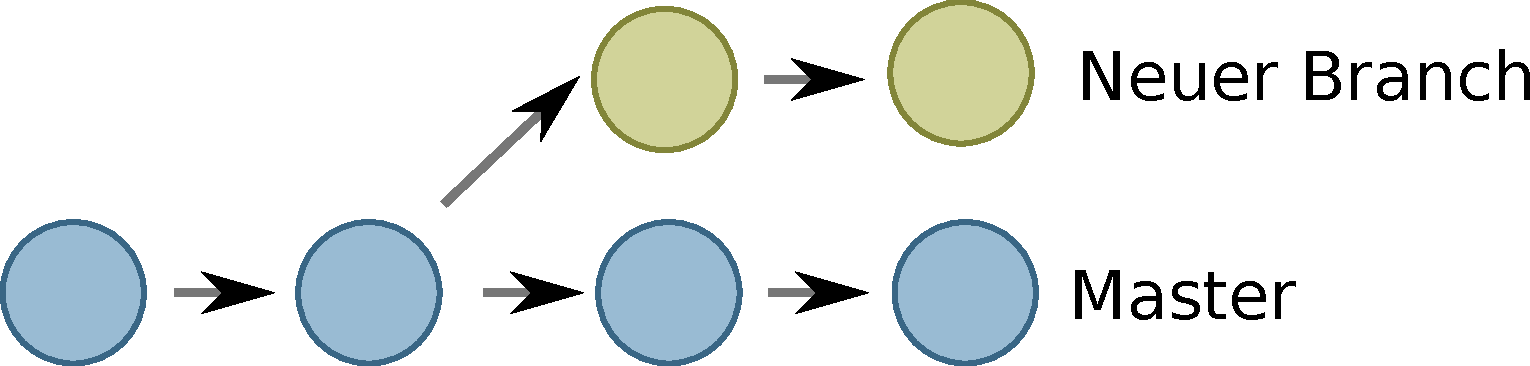
\includegraphics[width=7cm]{bilder/branch.pdf}
\end{center} 
%    \caption{}
%    \label{fig:awesome_image}
\end{figure}

Will man jedoch einen neuen Branch erstellen, um beispielweise ein neues Feature erst einmal nur für sich Programmieren will, so benutzt man

\begin{verbatim}
git checkout -b neuer_branch
\end{verbatim}

Wobei neuer\_ branch der Name des neuen Branches ist, den man erstellen will.

Um zum Master-Branch zurück zu welcheln verwendet man:
git checkout master

Einen Branch löschen Funktioniert mit:

\begin{verbatim}
git branch -d neuer_branch
\end{verbatim}

Der Branch ist jedoch noch nicht entfernt verfügbar sondern nur auf der lokalen Maschine.
Um den Branch anderen Verfügbar zu machen muss man ihn erst hochladen

\begin{verbatim}
git push origin <branch>
\end{verbatim}

Um Änderungen zu aktualisieren verwendet man hier ebenfalls git pull.

Will man den aktuellen Branch mit einem anderen zusammenführen, so verwendet man den
\begin{verbatim}
git merge <branch>
\end{verbatim}
Befehl.

Git versucht in beiden Fällen die Änderungen automatisch zusammenzuführen.
Ist dies nicht möglich, so muss man die Änderung selbst durchführen.

Git meldet in diesem Fall Konflikte.
Sind diese Konflikte aufgelöst, so kann man sie wieder mit

\begin{verbatim}
git add <dateiname> 
\end{verbatim}

stagen.

Mit 

\begin{verbatim}
git diff <quell_branch> <ziel_branch>
\end{verbatim}

lassen sie die Unterschiede näher betrachten.

\subsubsection{Zurücksetzen}
\marginpar{Kada}

\begin{figure}[htb]
\begin{center}
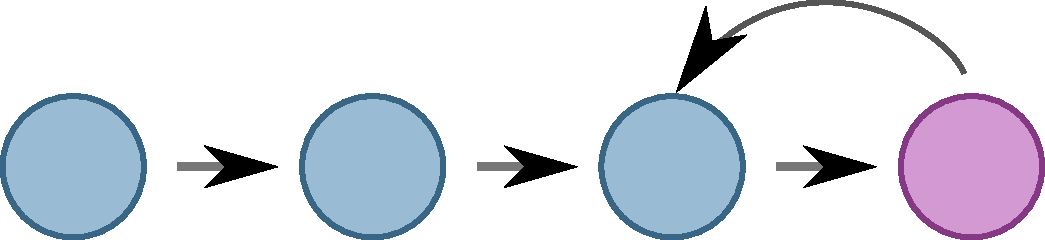
\includegraphics[width=7cm]{bilder/back.pdf}
\end{center} 
%    \caption{}
%    \label{fig:awesome_image}
\end{figure}
Für den den Fall, dass man lokale Änderungen wieder rückgängig machen möchte, kann man mit

\begin{verbatim}
git checkout --<filename>
\end{verbatim}

den Stand auf HEAD zurücksetzen lassen.

Sind die Änderungen bereits im Stage, so muss man sich eine Kopie aus demm entfernten Repository holen.
Die geschieht mit:

\begin{verbatim}
git fetch origin
git reset --hard origin/master
\end{verbatim}

\subsubsection{Forward}
\marginpar{Kada}

\begin{figure}[htb]
\begin{center}
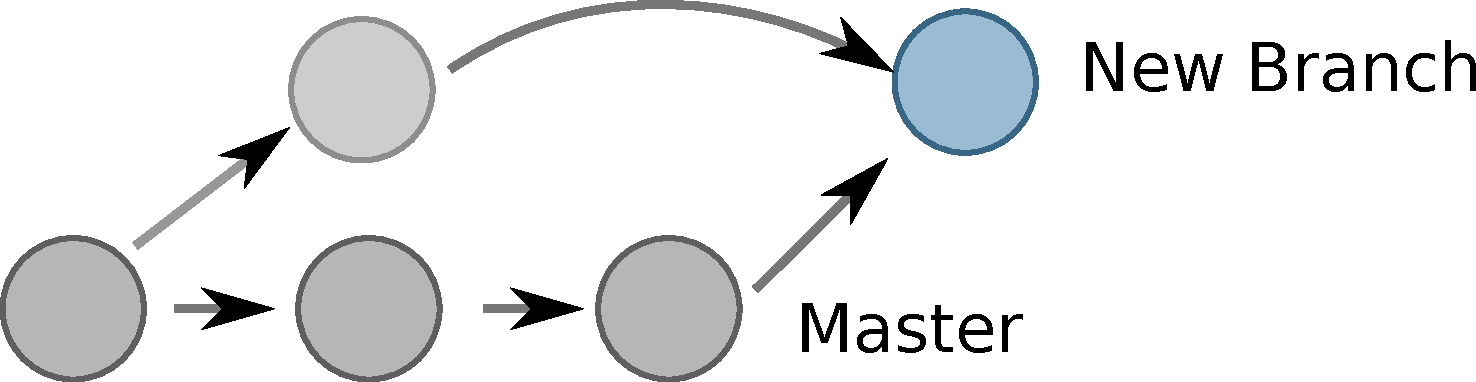
\includegraphics[width=7cm]{bilder/merge.pdf}
\end{center} 
%    \caption{}
%    \label{fig:awesome_image}
\end{figure}

\section{Programmiersprache und Hilfsmittel}

\subsection{C++}
\begin{itemize}
	\item kurze Beschreibung der Programmiersprache, Historie, etc
	\item Motivation, warum wir uns für C++ entschieden haben und nicht bspw. Python verwendet haben
\end{itemize}

\subsection{QT-Creator}
\begin{itemize}
	\item Motivation, warum wir dieses Programm einsetzen
	\begin{itemize}
		\item Plattformunabhängigkeit
		\item einfache Möglichkeit, eine GUI zu erstellen
	\end{itemize}
\end{itemize}

\subsection{SeqAn}
\marginpar{Benjamin}

SeqAn ist eine C++-Bibliothek zur Verarbeitung von biologischen Daten. Sie geht
auf ein Forchungsprojekt an der FU Berlin zurück und
stellt effiziente Algorithmen und Datenstrukturen zur verfügung, die auf
Sequenzen arbeiten. Die Bibliothek ist in C++ implementiert und auf Effizienz
und Erweiterbarkeit optimiert, was durch die rigorose Verwendung von
Template-Metaprogrammierung erreicht wird. Dies stellt auch gleichzeitig den
größten Nachteil von SeqAn dar, da einiges an Einarbeitung erforderlich ist um
mit dieser Programmierweise umgehen zu können.

Für die Projektgruppe hat sich SeqAn aus mehreren Gründen gegen andere
Bibliotheken durchgesetzt.

\begin{itemize}
	\item Unterstützung aller gängigen und von der Projektgruppe benötigten
          Dateiformate.
        \item Geschwindigkeit und Speicherverbrauch haben eine hohe Priorität.
	\item Sehr große Auswahl an Algorithmen mit dem sehr schnell
          Readmapper-Prototypen entwickelt werden können.
	\item Funktioniert auf vielen verschiedenen Plattformen, insbesondere
          auch unter Windows, was das Testen erleichtert.
\end{itemize}

Der Readmapper selbst benutzt SeqAn derzeit zur Ein- und Ausgabe von FASTA und
FASTQ-Dateien, das Auswerten von Kommandozeilenoptionen und die generelle
Behandlung von DNA-Strings. Hierbei haben sich die verschiedenen unterstützen
Alphabete wie DNA, DNA mit 'N' und Iupac als nützlich erwiesen. Die Algorithmen
werden derzeit nicht benutzt, da diese zu stark von den verbreiteten Verfahren,
die in SeqAn implementiert sind, abweichen.
